\chapter{作品整体设计方案}

\section{总体方案与平台边界}

MediFlow 把任务理解、领域编排和平台执行分成三个边界。Nexent 识别用户目标并选择任务级工具；MediFlow 校验参数、读取数据状态并选择处理流程；DataMate 执行数据集任务和单步算子，知识库与分析库负责持久化。当前三个智能体分别配置 5、11 和 8 项工具，去重后形成 17 个工具名称；工具在不同角色之间复用，但每个角色只暴露与其职责相关的入口。

三个阶段通过四类标识衔接：DataMate 数据集标识确定输入和交付数据集；任务一运行标识跟踪后台处理；任务二来源标识和记录标识定位文件与图谱记录；任务三分析标识关联问题、查询结果、图表和导出文件。
用户既可分别使用三个智能体，
也可将任务一产生的数据集直接交给任务二，
再由任务三读取图谱及分析表完成查询。

\section{系统分层与平台边界}

图~\ref{fig:architecture} 给出了作品的五层结构。
交互层包含 Nexent 对话入口和可视化工作台；智能体层按数据处理、知识构建和分析查询划分职责；接口层提供 MCP 工具和工作台业务接口；服务层由 DataMate 平台、医疗知识服务和分析服务组成；数据层保存交付数据集、知识图谱、分析数据库和导出文件。

\begin{figure}[H]
\centering
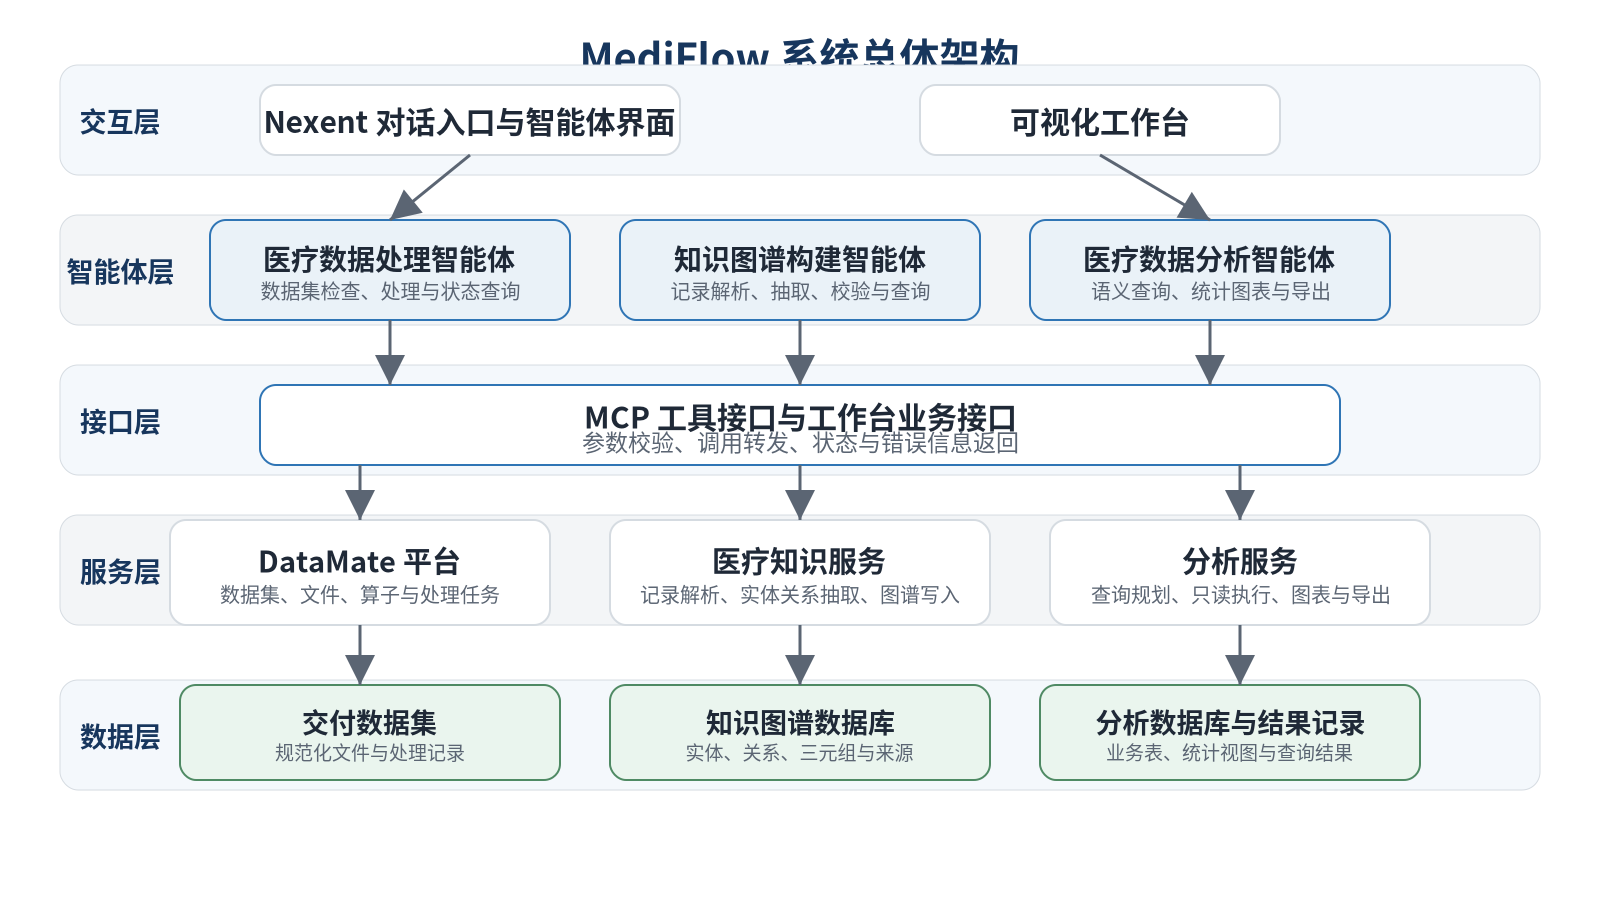
\includegraphics[width=0.98\textwidth]{figures/revision_architecture.png}
\caption{MediFlow 的分层架构与阶段数据对象}
\label{fig:architecture}
\end{figure}

DataMate 提供数据集、文件、算子和任务管理功能~\cite{datamate}。
Nexent 提供智能体配置、工具绑定、版本发布和对话执行功能~\cite{nexent,nexentdocs}。
项目使用 Model Context Protocol 连接 Nexent 与工具服务~\cite{mcpspec}，
在此基础上实现医疗格式路由、抽取校验、图谱持久化、查询安全和成果生成。
任务三还提供独立工作台入口，
它与 Nexent 查询工具共享图谱数据库和分析数据库，
用于集中呈现查询计划、关系图、统计图与成果下载。

\section{智能体工具调用机制}

智能体把用户任务转换为结构化工具调用，不直接执行文件处理、数据库写入或 SQL。图~\ref{fig:agent-call-chain} 展示一次调用的边界：Nexent 根据职责提示和工具说明识别任务类型，以工具名称和参数发起请求；FastMCP 将请求转交给 MediFlow 服务；服务按参数和数据状态选择处理流程，并把状态、产物标识和处理记录返回给智能体。

\begin{figure}[H]
\centering
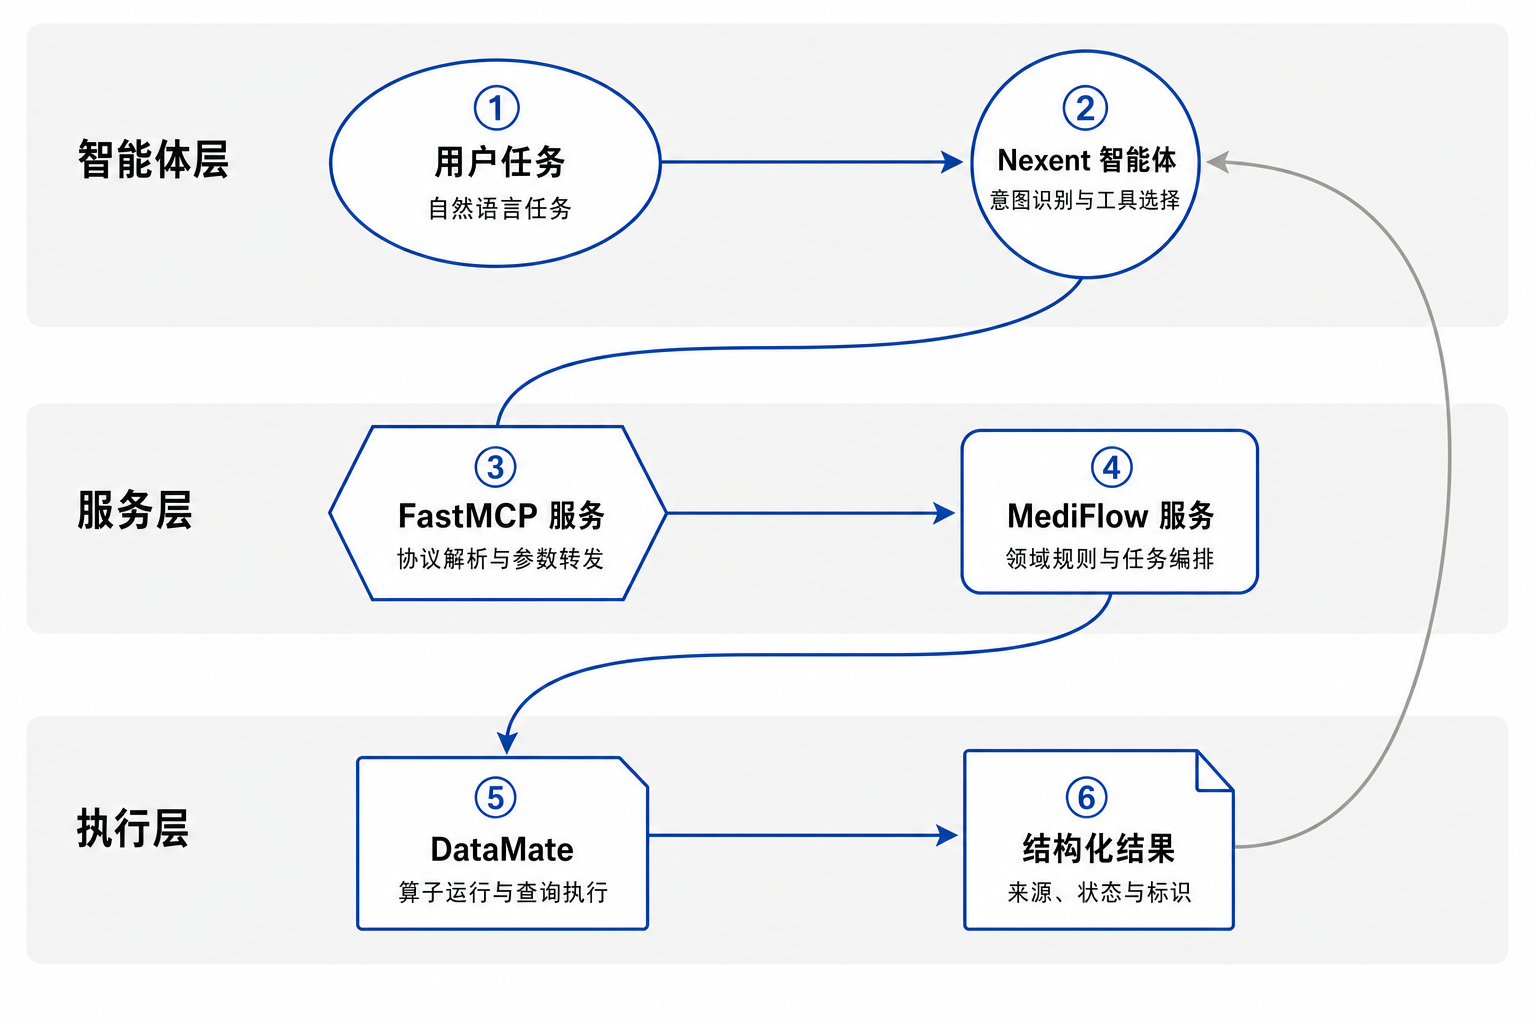
\includegraphics[width=0.96\textwidth]{figures/agent_call_chain_layered.png}
\caption{智能体单次调用的分层过程}
\label{fig:agent-call-chain}
\end{figure}

三个智能体使用不同的工具集合和职责规则。职责提示规定任务范围、工具调用顺序、参数来源和回复格式；约束提示规定只读边界、错误处理和禁止虚构结果；工具说明向模型提供接口名称、参数和返回字段。
模型据此选择任务级入口，
而不是直接决定每一个底层算子。
例如，任务一由智能体选择\texttt{run\_task1\_mixed\_cleaning}，
服务再按文件类型建立 DataMate 子任务和算子链。

工具返回的结构化状态决定后续动作。
小数据集完成后直接返回交付数据集，
大数据集返回运行标识并等待状态查询；
任务二返回抽取和入库状态，
任务三返回查询计划、数据行和分析标识。
工具调用失败时，智能体依据错误字段说明失败阶段和下一步，
实际产物以服务返回的状态和标识为准。

\begin{figure}[H]
\centering
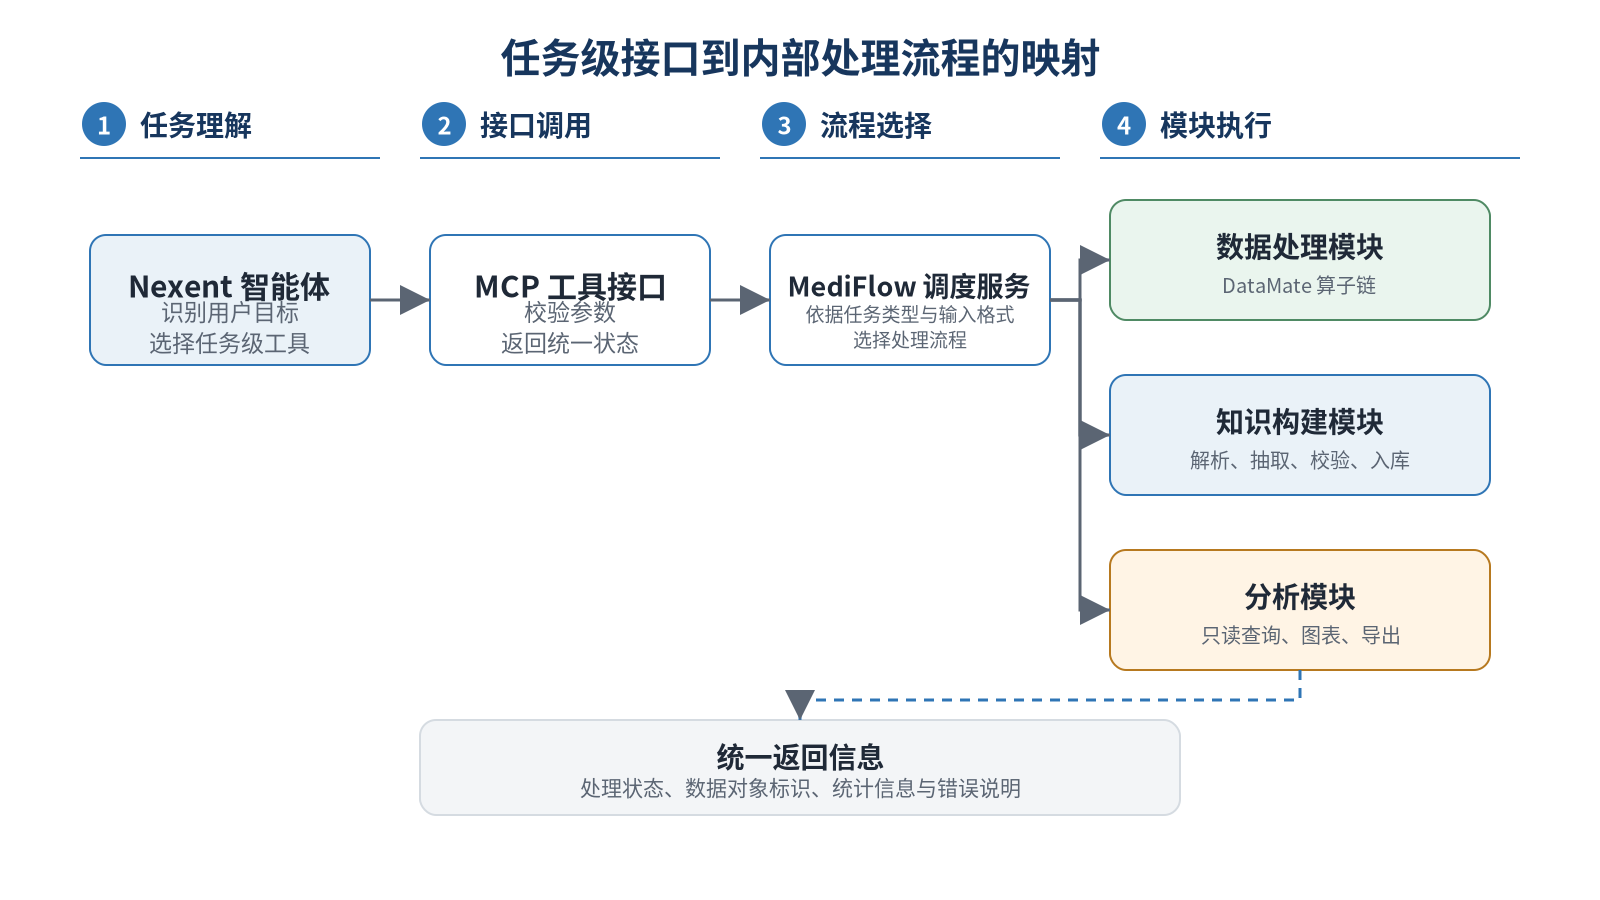
\includegraphics[width=0.96\textwidth]{figures/revision_task_mapping.png}
\caption{任务级工具到内部处理分支的映射}
\label{fig:task-interface-mapping}
\end{figure}

\subsection{DataMate 算子体系与执行边界}

DataMate 算子承担单步数据变换。项目算子采用 DataMate 的 Mapper 接口，由 \texttt{execute} 接收样本字典或文件记录，返回更新后的字段和处理记录；\texttt{metadata.yml} 保存注册信息。MediFlow 根据文件格式或抽取后端建立算子计划，DataMate 执行单步算子并返回结果；Nexent 只选择任务级 MCP 工具，不直接指定底层算子。

表~\ref{tab:operator-system} 归纳项目中的算子类别和执行边界。

\begin{table}[H]
\centering
\small
\caption{MediFlow 算子类别与执行边界}
\label{tab:operator-system}
\begin{tabularx}{\textwidth}{L{2.5cm}L{5.1cm}Y}
\toprule
\textbf{类别} & \textbf{代表算子} & \textbf{主要结果} \\
\midrule
通用清洗 &
EmojiCleaner、UrlRemover、WhitespaceNormalizer 等平台清洗算子 &
字符、链接、空白和文档噪声治理 \\
\addlinespace
医疗治理 &
MedicalTermNormalizer、MedicalTextQualityFilter、LLMNoiseFilter &
术语替换、质量筛选和噪声处理记录 \\
\addlinespace
结构保持 &
TableColumnCleaner、JsonFieldCleaner &
按字段清洗，保留表头、键名和嵌套层次 \\
\addlinespace
知识抽取 &
 MedicalEntityExtractor、MedicalRelationExtractor、MedicalTripleGenerator &
 实体关系抽取和三元组生成 \\
\addlinespace
记录组织 &
 MedicalRecordSplitter &
 按段落和句子边界拆分医疗记录，保留源文件与分段序号 \\
\addlinespace
统一输出 &
UnifiedJsonlExporter &
将多格式记录整理为任务二可读取的 JSONL \\
\bottomrule
\end{tabularx}
\end{table}

任务一在线流程直接创建 DataMate 清洗任务并轮询状态。
任务二的算子目录提供可注册的抽取资产，当前在线建图入口由
\texttt{run\_task2\_kg\_pipeline} 调用共享抽取服务，
再完成校验、入库和分析表刷新；两条路径共用实体关系模型和校验模块，
运行边界分别由 DataMate 任务和任务二领域服务负责。

图~\ref{fig:operator-execution} 将这条边界展开为一次完整调用：
智能体只选择任务级工具，服务再把参数映射为算子链或领域服务，
阶段产物统一回到带有状态和来源的结果记录。

\begin{figure}[H]
\centering
\begin{tikzpicture}[
  node distance=6mm and 7mm,
  main/.style={rectangle,draw=black!75,rounded corners=2pt,minimum width=3.0cm,
    minimum height=11mm,inner sep=3pt,align=center,font=\small,fill=blue!8},
  service/.style={rectangle,draw=black!75,rounded corners=2pt,minimum width=3.2cm,
    minimum height=11mm,inner sep=3pt,align=center,font=\small,fill=cyan!12},
  branch/.style={rectangle,draw=black!75,rounded corners=2pt,minimum width=3.2cm,
    minimum height=13mm,inner sep=3pt,align=center,font=\scriptsize},
  output/.style={rectangle,draw=black!75,rounded corners=2pt,minimum width=5.0cm,
    minimum height=10mm,inner sep=3pt,align=center,font=\small,fill=green!10},
  arrow/.style={-{Latex[length=1.8mm,width=1.1mm]},line width=0.65pt,
    draw=black!80,shorten <=2pt,shorten >=2pt},
  line/.style={line width=0.65pt,draw=black!80,shorten <=2pt,shorten >=2pt}
]
  \node[main] (agent) {Nexent 智能体\\任务理解与工具选择};
  \node[main,right=of agent] (mcp) {任务级 MCP 工具\\参数与状态边界};
  \node[service,right=of mcp] (service) {MediFlow 服务\\格式与后端映射};

  \node[service,below=9mm of service] (plan) {处理计划\\选择算子链或领域服务};
  \node[branch,fill=blue!8,below left=8mm and 6mm of plan] (task1)
    {任务一\\DataMate 清洗算子链};
  \node[branch,fill=blue!8,below=8mm of plan] (task2)
    {任务二\\抽取算子或共享服务};
  \node[branch,fill=gray!12,below right=8mm and 6mm of plan] (task3)
    {任务三\\只读分析查询服务};

  \node[output,below=8mm of task2] (output)
    {阶段产物与证据\\数据集、图谱事实、分析结果对象};

  \draw[arrow] (agent) -- (mcp);
  \draw[arrow] (mcp) -- (service);
  \draw[arrow] (service) -- (plan);

  \coordinate (branchpoint) at ($(plan.south)+(0,-3mm)$);
  \draw[line] (plan.south) -- (branchpoint);
  \draw[arrow] (branchpoint) -| (task1.north);
  \draw[arrow] (branchpoint) -- (task2.north);
  \draw[arrow] (branchpoint) -| (task3.north);

  \coordinate (outputpoint) at ($(output.north)+(0,3mm)$);
  \draw[line] (task1.south) |- (outputpoint);
  \draw[arrow] (task2.south) -- (output.north);
  \draw[line] (task3.south) |- (outputpoint);
\end{tikzpicture}

\caption{任务级工具到 DataMate 算子链的执行边界}
\label{fig:operator-execution}
\end{figure}

\section{智能体角色与工具配置}

项目按数据、知识和分析划分三个专业角色，
表~\ref{tab:agent-product-design} 从用户任务、执行逻辑和产物三个角度说明职责。Nexent 配置决定智能体可见的工具集合，MediFlow 服务负责参数校验和阶段内执行，DataMate 负责数据任务。
三个已发布角色覆盖赛题流程，自定义智能体也可复用其中的单项或组合工具。

\begin{table}[H]
\centering
\small
\caption{三个智能体的职责与工具边界}
\label{tab:agent-product-design}
\begin{tabularx}{\textwidth}{L{2.7cm}L{3.4cm}L{4.2cm}Y}
\toprule
\textbf{专业角色} & \textbf{用户任务} & \textbf{核心执行逻辑} & \textbf{主要产物} \\
\midrule
医疗数据处理 &
探查数据集、启动处理、查询进度、取得结果 &
识别五类文件，创建格式子数据集，运行 DataMate 算子链并汇聚结果 &
交付数据集、文件状态与处理报告 \\
\addlinespace
知识图谱生成与问答 &
从数据集建图、从文本抽取、查询疾病事实和关系 &
把文件解析为记录流，合并本地与模型抽取，校验后增量入库并刷新分析表 &
来源、实体、关系、三元组和疾病分析表 \\
\addlinespace
数据分析与可视化 &
查询疾病属性、统计关系分布、核对来源、导出分析成果 &
优先使用医疗语义模板规划查询，校验只读 SQL，组织回答、图表和报告 &
分析结果记录与 HTML、CSV、JSON 成果包 \\
\bottomrule
\end{tabularx}
\end{table}

\section{阶段数据与存储设计}

系统根据数据的使用方式设置三类存储。
DataMate 保存待处理文件、算子任务和交付数据集；
知识图谱 SQLite 库保存规范化实体关系及其来源；
分析 SQLite 库保存面向疾病查询的关系表和统计视图。
任务三执行过程中生成一条分析结果记录。表~\ref{tab:data-contract} 列出各层的实际结构。

\begin{table}[H]
\centering
\caption{核心存储与阶段数据对象}
\label{tab:data-contract}
\begin{tabularx}{\textwidth}{L{2.8cm}L{5.0cm}Y}
\toprule
\textbf{对象} & \textbf{主要结构} & \textbf{作用} \\
\midrule
DataMate 数据集 &
数据集标识、文件清单、算子实例、清洗任务、目标数据集 &
承载任务一输入、分格式处理和最终交付 \\
\addlinespace
知识图谱库 &
\texttt{kg\_sources}、\texttt{kg\_entities}、\texttt{kg\_aliases}、
\texttt{kg\_relations}、\texttt{kg\_triples}、\texttt{kg\_quality\_issues} &
保存实体关系、原文片段、来源和质量记录 \\
\addlinespace
分析数据库 &
\texttt{diseases}、\texttt{disease\_facts}、9 张疾病关系表、
统计表与统计视图 &
支持疾病属性查询、分布统计和图表生成 \\
\addlinespace
分析结果记录 &
分析标识、问题、查询计划、SQL、数据行、图表配置和来源信息 &
统一驱动文字回答、结果表、图表和成果导出 \\
\bottomrule
\end{tabularx}
\end{table}

知识图谱库适合维护规范化实体、关系和事实来源，
分析数据库则按关系类型把三元组转换为疾病与症状、药物、检查、科室等直接可查的业务表。
这种双库结构使任务二可以按事实粒度增量写入，
任务三可以使用简单、稳定的 SQL 完成聚合查询。

\section{跨阶段执行链路}

一次完整业务过程由以下六步组成：

\begin{enumerate}
  \item 用户在 DataMate 准备资料数据集，数据处理智能体先读取文件清单与格式分布；
  \item 任务一按格式建立子数据集，执行相应算子链，并登记新的交付数据集；
  \item 任务二按源文件轮转读取记录，避免处理上限集中落在单个文件；
  \item 抽取结果经实体位置、类型、关系引用和置信度校验后写入图谱事务；
  \item 新增三元组写入成功后刷新疾病事实表、九类关系表和统计视图；
  \item 任务三使用语义模板或经过约束的查询计划访问分析库，生成回答、数据表、图表和导出文件。
\end{enumerate}

这套流程允许单独运行任一任务。
已有公开医学资源可直接构成基础知识图谱，
新接入资料则沿任务一、任务二进入同一图谱，
任务三使用统一的数据口径展示已有知识与新增知识。

\section{结果校验与安全边界}

任务一在结果汇聚前重新解析 JSON、JSONL 和 CSV 产物，
PDF 分支分别保存上传、解析、下载和正文转换状态；
文件数超过 50 时转为后台任务并返回运行标识。
任务二只接收九类医疗实体和关系映射表中的关系，实体必须能在原文中定位。抽取结果先按可靠性等级分为高、中、低三级，再分别进入主图谱、候选记录或拦截记录；通用三元组转换函数的 0.7 参数是默认下限，在线级联入口显式保留候选，由持久化规则完成最终分流。
任务三只允许访问预先登记的 17 张表和视图，
SQL 必须为单条 \texttt{SELECT} 或 \texttt{WITH} 语句，
数据库连接启用只读与 \texttt{query\_only}，
单次最多执行 4 项查询、每项最多返回 200 行并设置 5 秒中止条件。
这些控制直接嵌入处理链和数据库访问层，
对 Nexent 入口与独立工作台采用同一执行规则。
